%% Document created 28 April 2021 automatically 
%% from /Users/massimosotgia/Desktop/uni_at_DIFI/Lab_C03/setup.py 

%% Copyright (C) Mattia Sotgia et al. 2021
%% Using class lab_unige.cls
%                                                            
%                                                            
%   **                 **             ******   ****   ****   
%  /**                /**            **////** *///** */// *  
%  /**        ******  /**           **    // /*  */*/    /*  
%  /**       ´´´´´´** /******      /**       /* * /*   ***   
%  /**        ******* /**///**     /**       /**  /*  /// *  
%  /**       **´´´´** /**  /** **  //**    **/*   /* *   /*  
%  /********//********/****** /**   //****** / **** / ****   
%  ////////  //////// /////   //     //////   ////   /´///   
%                                                            
%                                                            
\documentclass[italian, a4paper, 10pt, twocolumn]{../../style/lab_unige}
\usepackage[a4paper, margin=1.75cm, footskip=0.25in]{geometry}

\usepackage[utf8]{inputenc}
\usepackage[T1]{fontenc}

\usepackage[italian]{babel}

% \usepackage{biblatex}

\usepackage[bookmarksopen=true, citebordercolor={0 1 0}, linkbordercolor={1 0 0}, urlbordercolor={0 1 1}]{hyperref}
\usepackage[numbered]{bookmark}

\usepackage{graphicx}
\graphicspath{{../fig/}}
\usepackage{array}
\usepackage{tabulary}
\usepackage{booktabs}

% FOUNDAMENTAL
\usepackage{../../style/custom}

\usepackage{physics}

\usepackage{breqn}
\usepackage{cuted}
\usepackage{txfonts}

\usepackage{lipsum}

\usepackage[american resistors]{circuitikz}

%% Define ref types
\newcommand{\reftab}[1]{Tabella {\ref{#1}}}%
\newcommand{\reffig}[1]{Figura {\ref{#1}}}%
\newcommand{\refeqn}[1]{Eq. ({\ref{#1}})}%
\newcommand{\ChiSqr}{$\chi^2$\space}
\newcommand{\ChiNdf}{$\chi^2/\text{ndf}$}
\newcommand{\cernroot}{\texttt{root}}
\newcommand{\treSigma}{$3\sigma$}
\newcommand{\stdErr}[1]{$\varepsilon_{#1}$}
\newcommand{\mstdErr}[1]{\varepsilon_{#1}}
\newcommand{\gLab}{$g_t~=~(~9.8056~\pm~0.0001~\text{ stat}~)~\text{ m/s}^2$}
%% PAPER ONLY custom Macros


%%
\setlength{\columnsep}{6mm}

\begin{document}
    \twocolumn[
    \begin{@twocolumnfalse}
        \title{
            Metodo Volt-Amperometrico E Circuito RC 
        }
        \author{
        Eugenio Dormicchi\textsuperscript{1, 2},
        % Riccardo Pizzimbone\textsuperscript{1}, 
        Giovanni Oliveri\textsuperscript{1},
        Mattia Sotgia\textsuperscript{1}
        }

        \date{
            \textit{
            \textsuperscript{1}Gruppo C03, Esperienza di laboratorio n. 8 \\
            \textsuperscript{2}In presenza in laboratorio per la presa dati\\
            }
            % Università degli Studi di Genova, Dipartimento di Fisica.\\
            \vspace{2ex}
            (Presa dati
            28 Aprile 2021, 15:00– 18:00; Analisi dati 
            4 Maggio 2021)
        }
        \maketitle
        
        \begin{abstract}
            \textit{Obiettivo-- }
            Vogliamo misurare con il metodo voltamperometrico il valore delle resistenze $R_1$ e $R_2$ e successivamente la capacità $C$ di un condensatore mediante la misura della costante di tempo caratteristica di un circuito RC $\tau$.
            \textit{Metodi-- }
            Circuiti elettrici, carica e scarica condensatori, Fit polinomiali ed esponenziali. 
            \textit{Risultati-- }
            Troviamo i valori di $R_1$ e $R_2$, ottenendo anche un andamento lineare che indica una proporzionalità diretta tra $I$ e $V$. Osserviamo un andamento esponenziale coerente con la teoria per i processi di carica e scarica di un condensatore.
            \textit{Conclusione-- }
            I valori delle resistenze sono compatibili con quelli misurati. Invece per la seconda parte dell'esperienza osserviamo che invece i modelli nonostante mostrino un andamento esponenziale, non siano effettivamente compatibili con quelli teorici.
        
        \end{abstract}
        \vspace{2em}
    \end{@twocolumnfalse}
    ]

    %%%% CORPO DEL TESTO
    %%%% CORPO DEL TESTO

    \section{Introduzione}
    \label{section:introduction}

    Si vuole misurare il valore delle resistenze $R_1$ e $R_2$ sfruttando il metodo voltamperometrico, e poi misurare la capacità di un condensatore, a partire dalla misura della costante di tempo su un circuito RC. 

    \subsection{Metodo voltamperometrico}

    Il metodo voltamperometrico è un processo sperimentale, che consente di risalire al valore di una resistenza, tramite le misure della tensione ai suoi capi, e dell’intensità di corrente fluente al suo interno. Chiamando $I_R$ la corrente che scorre all’interno della resistenza, e $V_R$ la tensione ai suoi estremi, possiamo calcolare il valore della resistenza $R$, con la formula \[R=\frac{V_R}{I_R}.\]

    Nella prima parte dell’esperienza, misuriamo i valori di due resistenze $R_1$ e $R_2$, mediante il metodo voltamperometrico.

    Il circuito realizzato è composto da un generatore, collegato ad una resistenza nel circuito primario. Sullo stesso circuito è collegato l'amperometro, e in parallelo alla resistenza (posta dopo l'amperometro) è posizionato il voltmetro.
    Il  circuito sul quale sono effettuate le misure è mostrato in \reffig{figure:VI_circ}. 

    \begin{figure}[h!]
        \centering
        \begin{circuitikz} \draw
            (0,4) -- (1,4)
            (1,4) to [ammeter, l=$I_A$, *-](4,4)
            (4,4) -- (6,4)
            (0,4) to [V<=$V_0$](0,0)
            (0,0) -- (6,0)
            (6,0) to [voltmeter, l=$V_V$, rotate=0](6,4)
            (4,0) to [R, l=$R$, *-*](4,4)
            ;
        \end{circuitikz}
        \caption{Schema elettrico del circuito utilizzato per la misura delle resistenze $R_1$ e $R_2$ con il metodo voltamperometrico.}
        \label{figure:VI_circ}
    \end{figure}
    

    \subsection{Circuito RC}
    
    La seconda parte dell’esperienza si concentrata sullo studio dei processi di carica e scarica di un condensatore in due circuiti RC, in ciascuno dei quali è presente una delle resistenze considerate nella prima parte dell'esperienza. \\
    Il circuito RC è un circuito elettrico semplice, nel quale sono presenti un resistore $R$ e un condensatore $C$ montati in serie; nel circuito è inoltre presente un commutatore posto tra il polo positivo del generatore di tensione e la resistenza $R$. Il commutatore serve per includere ed escludere il generatore dal circuito. Studiando il processo di carica di un condensatore, si può misurare la costante di tempo ($\tau$) del circuito: un valore di tempo indicativo della velocità con la quale avviene il processo di carica.

    La misura della costante di tempo viene effettuata grazie alla variazione di tensioni ai capi della capacità durante la chiusura o l’apertura dell’interruttore.
    La carica del condensatore avviene commutando l’interruttore, al tempo $t_0$, in modo da includere il generatore di corrente nel circuito; la tensione $V_C$ ai capi del condensatore avrà l’andamento seguente
    \begin{equation}
        V_C(t)=V_\infty\left(1-e^{-\frac{t-t_0}{\tau}}\right) \label{equation:carica}
    \end{equation}
    dove $\tau=RC$ è la costante caratteristica di tempo del circuito. Quando il condensatore sarà completamente carico la tensione raggiungerà un valore costante $V_\infty$ che sarà pari a $V_0$ del generatore nel caso ideale in cui il voltmetro ha resistenza interna infinita.

    Successivamente al processo di carica del condensatore spostiamo l’interruttore, scollegando il circuito dal generatore, al tempo $t=0$, affinché il generatore venga escluso dal circuito.
    La tensione VC ai capi del condensatore avrà il seguente andamento
    \begin{equation}
        V_C(t) = V_Ie^{-\frac{t}{\tau}} \label{equation:scarica}
    \end{equation}

    Dove $\tau$ è la stessa costante di tempo del processo di carica e $V_I$ è la tensione ai capi del condensatore  nell’istante in cui viene commutato l’interruttore che quindi sarà inferiore alla tensione di regime.

    \begin{figure}[h!]
        \centering
        \begin{circuitikz} \draw
            (0,4) to [short, -*] (1.2,4) node[above] {A}
            (1.5, 0) to[short, -*](1.5, 3.5) node[right] {B}
            (5.2,4) to [R, l_=$R$, *-*](2,4) node[above] {T}
            (2,4) -- (1.35, 3.75) 
            (0,4) to [V<=1V](0,0)
            (0,0) to[short, -*] (5.2,0)
            (5.35,0) to[short, *-] (6,0)
            (5.35,4) to[short, *-] (6,4)
            (6,0) to [voltmeter, l_=$V_C(t)$](6,4)
            (4.5,0) to [C, l=$C$](4.5,4)
            ;
            \draw (-0.5, 2) node[left] {$V_0$}
            ;
        \end{circuitikz}
        \caption{Schema elettrico del circuito utilizzato nella seconda parte dell'esperienza. Troviamo indicato con T il commutatore che può chiudere il circuito con A o con B, escludendo o meno il generatore.}
        \label{figure:RC_circ}
    \end{figure}


    % \section{Strumentazione}
    % \label{section:strument}

    \section{Metodi}
    \label{section:methods}

    \subsection{Metodo voltamperometrico}

    La prima parte dell’esperienza consiste nel misurare due resistenze attraverso il metodo voltamperometrico. Quest’ultimo rappresenta un modo indiretto di misurazione di resistenze elettriche ed è bastato sulla legge di Ohm.\\
    Il metodo voltamperometrico necessita di un circuito costituito da un generatore di tensione continua che alimenti la resistenza incognita, un amperometro e un voltmetro. Più la resistenza che si intende misurare è piccola più è necessario che la corrente non sia eccessivamente grande per non compromettere la struttura della resistenza e del circuito stesso.

    Esistono due metodi voltamperometrici distinti: metodo voltamperometrico con voltmetro a valle e metodo voltamperometrico con voltmetro a monte.\\
    Nella nostra esperienza faremo riferimento alla configurazione con voltmetro posizionato a valle dell’ amperometro \reffig{figure:VI_circ}.\\
    In questa situazione il voltmetro misura la tensione ai capi della resistenza incognita e l’amperometro misura la corrente che circola nella resistenza interna sommata a quella  che permette il funzionamento del voltmetro.\\
    Questo metodo è efficace se la resistenza del voltmetro è molto maggiore della resistenza incognita poiché la resistenza equivalente di due resistenze poste in parallelo è $R_{eq}=(R_V R)/(R_V+R)$ (dove $R$ è la resistenza incognita e $R_V$ è quella del voltmetro).
    Considerando trascurabili gli effetti dovute alle resistenze interne degli strumenti, si ottiene $I_A$ circa $I_R$ e $V_V$ circa $V_R$. 
    Variando la tensione $V_0$ del generatore è possibile misurare coppie di valori $V_V$ e $I_A$.  I valori misurati sono legati dalla relazione lineare \begin{equation}
        V_V =RI_A \label{equation:VI}
    \end{equation} di conseguenza è possibile ottenere $R$ incognita.

    Il circuito sulla basetta è stato già predisposto dai docenti, il nostro primo scopo è collegare in modo corretto il circuito al generatore, al  multimetro da banco e al Tester.
    Per la prima parte è necessario che il multimetro da banco sia impostato in modalità di lettura di correnti continue (tasto DC) mentre il tester sia impostato in modalità di lettura di tensioni continue.\\
    Utilizziamo l’Output-1 del generatore collegando l’uscita positiva di quest’ultimo  all’amperometro nella boccola dei milliAmpere attraverso un cavo schermato. Un secondo cavo uscente dal foro comune dell’amperometro viene mandato ai capi della resistenza cioè al terminale giallo andando così a costituire la corrente entrante; infine colleghiamo l’ingresso nero con un terzo filo (di diverso colore per distinguerlo dai precedenti) all’uscita negativa del generatore, chiudendo così il circuito.

    Successivamente colleghiamo il nostro tester, che svolgerà la funzione di voltmetro, in parallelo alla resistenza.\\
    Esso dispone di un foro centrale, che costituisce l’uscita comune, e a destra di quest’ultimo un secondo foro per le tensioni continue. Colleghiamo quindi l’uscita delle tensioni del tester dietro al cavo dell’amperometro (boccola gialla) mentre il cavo di ritorno nero dietro la boccola nera fino all'entrata comune (COM) del tester.\\
    Per sicurezza si può utilizzare il comando Display Limit così di limitare la potenza erogata dal generatore e non danneggiare il circuito.

    Per ciascuna delle due resistenze eseguiamo i seguenti passaggi: inizialmente montiamo la resistenza incognita  all’ interno del circuito facendo attenzione che il generatore non stia erogando tensione. Successivamente effettuiamo 6  coppie misure di $V_V$ e $I_A$ variando la tensione $V_0$ erogata dal generatore in un intervallo da 0~V fino a 10~V.  

    Tutte le misure vanno fatte utilizzando il fondo scala più appropriato per ciascuno strumento e della misura che si effettua; ci segniamo di volta in volta il fondo scala utilizzato: questo permetterà di associare ai valori le relative incertezze deducibili dai data-sheet. Infine eseguiamo un fit lineare e ricaviamo il valore delle due resistenze $R_1$ e $R_2$.

    \subsection{Circuito RC}

    Inizialmente il nostro compito è collegare correttamente il circuito al multimetro da banco, impostato in modalità di lettura di tensioni continue, e al generatore di corrente.\\
    Congiungiamo il circuito al generatore: l’uscita negativa di quest’ultimo viene collegata alla boccola nera mentre quella positiva viene collegata al terminale rosso della basetta.\\
    Successivamente scolleghiamo il tester e andiamo a collegare il multimetro da banco che svolgerà la funzione di voltmetro.

    Colleghiamo attraverso un cavo l’uscita COM del multimetro alla boccola nera della basetta mentre con un secondo cavo attacchiamo l’uscita della tensione positiva all’ingresso verde. Prima di procedere alla presa dati è importante verificare che il multimetro sia impostato correttamente in lettura di tensioni continue, selezionando il tasto DCV; inoltre è necessario selezionare il fondo scala dei 2~Volt e impostarlo in \verb|manual range|. Infine montiamo la resistenza misurata in precedenza posizionandola nei fori corretti sulla basetta.

    Dopo aver verificato che il tutto sia montato correttamente si può procedere con la seconda parte dell’ esperienza.

    Questa consiste nell’ utilizzo delle due resistenze misurate precedentemente all’ interno del circuito descritto sopra di cui dobbiamo trovare la constante di tempo nel processo di carica e scarica.

    La misura viene effettuata attraverso il programma DMMDaq che acquisisce a intervalli di tempo costanti la tensione letta dal multimetro da banco. Per ciascuna misura è necessario acquisire dati per una durata pari a circa 2-3 costanti di tempo da quando l’interruttore viene commutato.  Scegliamo infine una frequenza di acquisizione appropriata in modo da ottenere circa 5-10 misure per ogni costante di tempo. 

    Procediamo quindi con la misura di carica: impostiamo la tensione del generatore ad un valore compreso tra i 0.2~V e i 2~V che verrà mantenuta costante durante la misura; nel nostro caso abbiamo selezionato una tensione costante erogata dal generatore $1$~V.\\
    Commutiamo l’interruttore in modo da escludere il generatore e attendiamo sufficientemente a lungo finché la tensione letta dal multimetro  sia compatibile con zero. 

    Successivamente facciamo partire il programma dal terminale e gli forniamo i comandi seguenti: \verb|T|, \verb|t|, nome del file in cui salvare i dati e intervallo di tempo di acquisizione $\Delta t$. 

    Per la prima resistenza è conveniente scegliere un $\Delta t$ di 0.5~s mentre per la seconda un intervallo di 1~s. Appena dopo aver fatto partire l’ acquisizione spostiamo l'interruttore così da includere il generatore e interrompiamo la presa dati dopo circa 2-3 costanti di tempo del circuito (45 secondi per la prima resistenza e 90 secondi per la seconda, stimando come costanti di tempo $\tau_1\approx$10~s e $\tau_2\approx$30~s).

    Completata la misura di carica procediamo con quella di scarica mantenendo sempre il circuito in tensione:  prepariamo il programma di acquisizione dati inserendo gli stessi comandi dati in precedenza e lo stesso intervallo di tempo tra due misure successive usato per il processo di carica. \\
    Commutiamo l’ interruttore escludendo il generatore e immediatamente dopo facciamo partire  l’acquisizione dati. Analogamente a prima interrompiamo il programma dopo un tempo circa pari a 2-3~$\tau$.
    Dopo aver concluso le misure di carica e scarica del circuito RC utilizzando la resistenza $R_1$, procediamo con la resistenza $R_2$ ripetendo i medesimi passaggi.

    Come controllo finale è possibile misurare direttamente le resistenze impostando il multimetro in modalità ohmmetro. \\
    Scolleghiamo quindi le parti del circuito non essenziali, collegando infine la boccola nera all’ uscita comune del multimetro e la boccola rossa al foro di lettura delle resistenze. \\
    I valori delle resistenze così ottenuti sono $R_1^m=(9.9371\pm0.0015)$~k$\Omega$ e $R_2^m=(32.770\pm0.007)$~k$\Omega$, dove gli errori sono statistici e ottenuti dal data-sheet del multimetro da banco come
    \[\mstdErr{R}=\frac{0.002\% \cdot val + 0.003\% * range}{\sqrt{3}}~~~(\text{range}=20/200~\text{k}\Omega).\]

    I valori forniti dal multimetro dovranno essere poi confrontati con quelli ottenuti attraverso il metodo voltamperometrico (si vedano le Conclusioni \ref{section:conclusion}).


    \section{Analisi dati}
    \label{section:analysis}

    \subsection{Stima delle resistenze}

    Rappresentiamo le coppie ($I_A$, $V_V$) trascritte in \reftab{table:R1} e \reftab{table:R2} nella \reffig{figure:plot_R1_R2}, dove possiamo osservare un andamento lineare. Per le coppie ($I_A$, $V_V$) consideriamo come incertezza il valore deducibile dal data-sheet.\\
    Per la corrente $I_A$ l'errore 
    \[
        \mstdErr{I_A} =
            \begin{cases}
                \frac{0.03\%\cdot val + 0.05\%\cdot range}{\sqrt{3}} & \text{(se range}=200~\mu\text{A)}\\
                \frac{0.02\%\cdot val + 0.05\%\cdot range}{\sqrt{3}} & \text{(se range}=2~\text{mA)}
            \end{cases}
    \]
    mentre per la tensione il valore è
    \[
        \mstdErr{V_V} =
            \begin{cases}
                \frac{0.015\%\cdot val+0.001}{\sqrt{3}} & (\text{se range}=2~V)\\
                \frac{0.015\%\cdot val+0.01 }{\sqrt{3}} & (\text{se range}=20~V)
            \end{cases}
    \]
    dove \textit{range} indica il fondo scala scelto, \textit{val} indica il valore letto dallo strumento.

    \begin{figure}
        \centering
        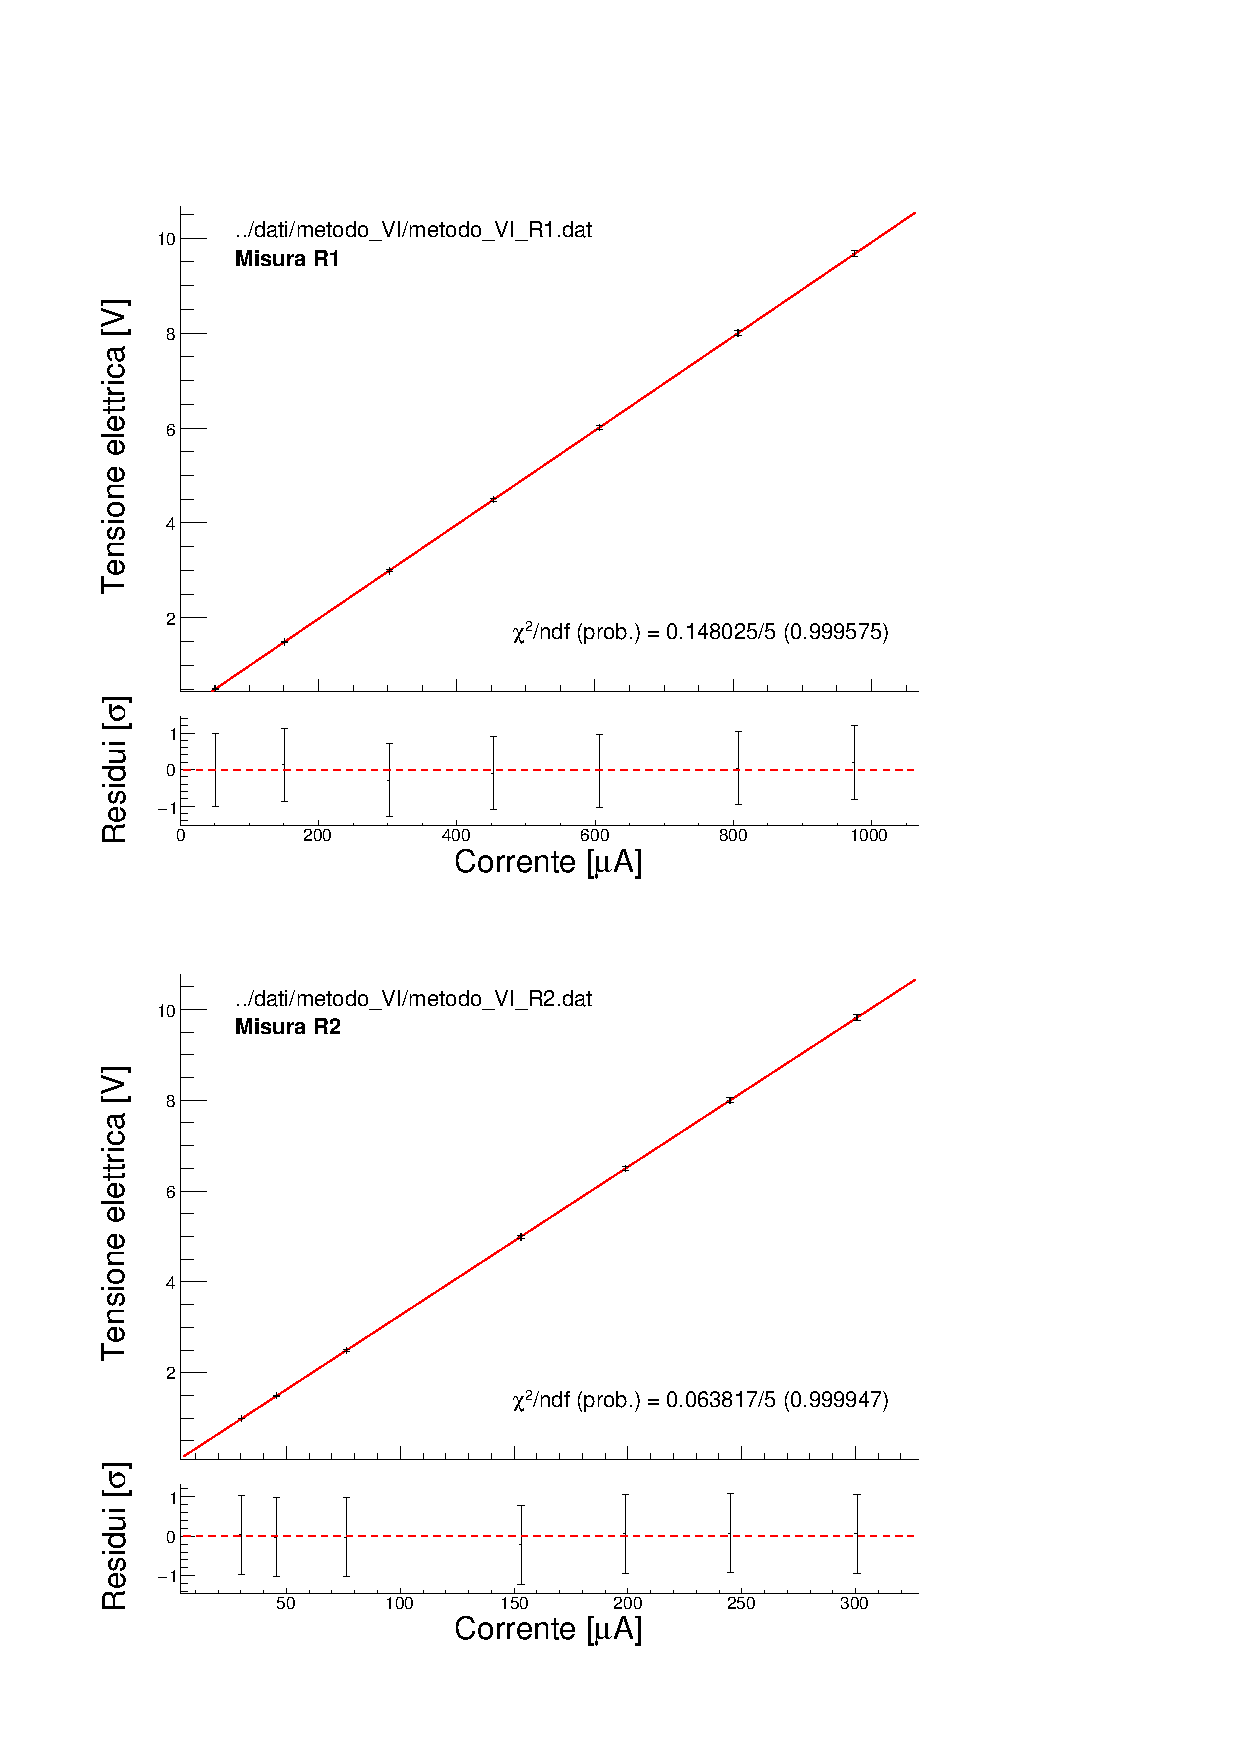
\includegraphics[width=\linewidth]{misura_R1_R2.pdf}
        \caption{Grafico delle coppie di punti ($I_A$, $V_V$) misurati nella prima parte dell'esperienza, con i relativi residui. Sopra sono rappresentati i punti delle misure relativi a $R_1$, sotto troviamo i valori relativi alla misura di $R_2$. Il valore del \ChiSqr, e il valore del rapporto \ChiNdf, indicano in entrambi i casi un Fit quasi troppo perfetto, potremmo quindi ipotizzare di aver sovrastimato gli errori, osservando comunque che tutti i punti sono vicini al valor vero a meno di $1\sigma$.}
        \label{figure:plot_R1_R2}
    \end{figure}

    Dalla \refeqn{equation:VI} possiamo ricavare una relazione lineare rappresentabile da una polinomiale di primo grado (\verb|pol1| in \cernroot) come $a_0 + a_1x = y$, dove $a_0$ deve essere compatibile con 0.\\
    Dal Fit possiamo ricavare una stima di $R_1$ e $R_2$. In \reffig{equation:VI} rappresentiamo anche i grafici dei residui, dove il valore sulle $x$ è lo stesso, mentre sulle $y$ poniamo
    \[
        \frac{V_{\text{misurata}}-V_{fit}}{\mstdErr{V_{\text{misurata}}}}.
    \]
    che rappresenta lo spostamento del valore misurato dal Fit, normalizzato, a cui è associato un errore pari a $1\sigma$. In questa considerazione stiamo assumendo che la distribuzione di probabilità dei singoli punti sia Gaussiana.

    \begin{table}
    \centering
    \footnotesize
    \caption{Coppie di valori ($I_A$, $V_V$) del circuito con $R_1$.}
    \label{table:R1}
    \begin{tabular}{lcc}
        \hline\hline\\[-1.5ex]
          & Corrente Elettrica [$\mu$A] & Tensione Elettrica [V] \\[+0.5ex] \hline \\[-1.5ex]
        1 & $50.688\pm0.015$            & $0.502\pm0.003$        \\[+0.5ex]
        2 & $150.36\pm0.03 $            & $1.491\pm0.009$        \\[+0.5ex]
        3 & $302.39\pm0.09 $            & $2.99 \pm0.023$        \\[+0.5ex]
        4 & $453.40\pm0.11 $            & $4.49 \pm0.03 $        \\[+0.5ex]
        5 & $606.57\pm0.13 $            & $6.01 \pm0.04 $        \\[+0.5ex]
        6 & $807.01\pm0.15 $            & $8.00 \pm0.05 $        \\[+0.5ex]
        7 & $975.54\pm0.17 $            & $9.68 \pm0.06 $        \\[+0.5ex] \hline \\[-1.5ex]   
    \end{tabular}
\end{table}

\begin{table}
    \centering
    \footnotesize
    \caption{Coppie di valori ($I_A$, $V_V$) del circuito con $R_2$.}
    \label{table:R2}
    \begin{tabular}{lcc}
        \hline\hline\\[-1.5ex]
          & Corrente Elettrica [$\mu$A] & Tensione Elettrica [V] \\[+0.5ex] \hline \\[-1.5ex]
        1 & $30.395\pm0.011$            & $0.992\pm 0.006$        \\[+0.5ex]
        2 & $45.692\pm0.014$            & $1.491\pm 0.009$        \\[+0.5ex]
        3 & $76.296\pm0.019$            & $2.49 \pm 0.02 $        \\[+0.5ex]
        4 & $153.08\pm0.03 $            & $4.99 \pm 0.03 $        \\[+0.5ex]
        5 & $199.00\pm0.04 $            & $6.50 \pm 0.04 $        \\[+0.5ex]
        6 & $244.91\pm0.09 $            & $8.00 \pm 0.05 $        \\[+0.5ex]
        7 & $300.65\pm0.09 $            & $9.82 \pm 0.06 $        \\[+0.5ex] \hline \\[-1.5ex]   
    \end{tabular}
\end{table}



    \subsection{Stima delle costanti di tempo}

    \begin{figure*}[t!]
        \centering
        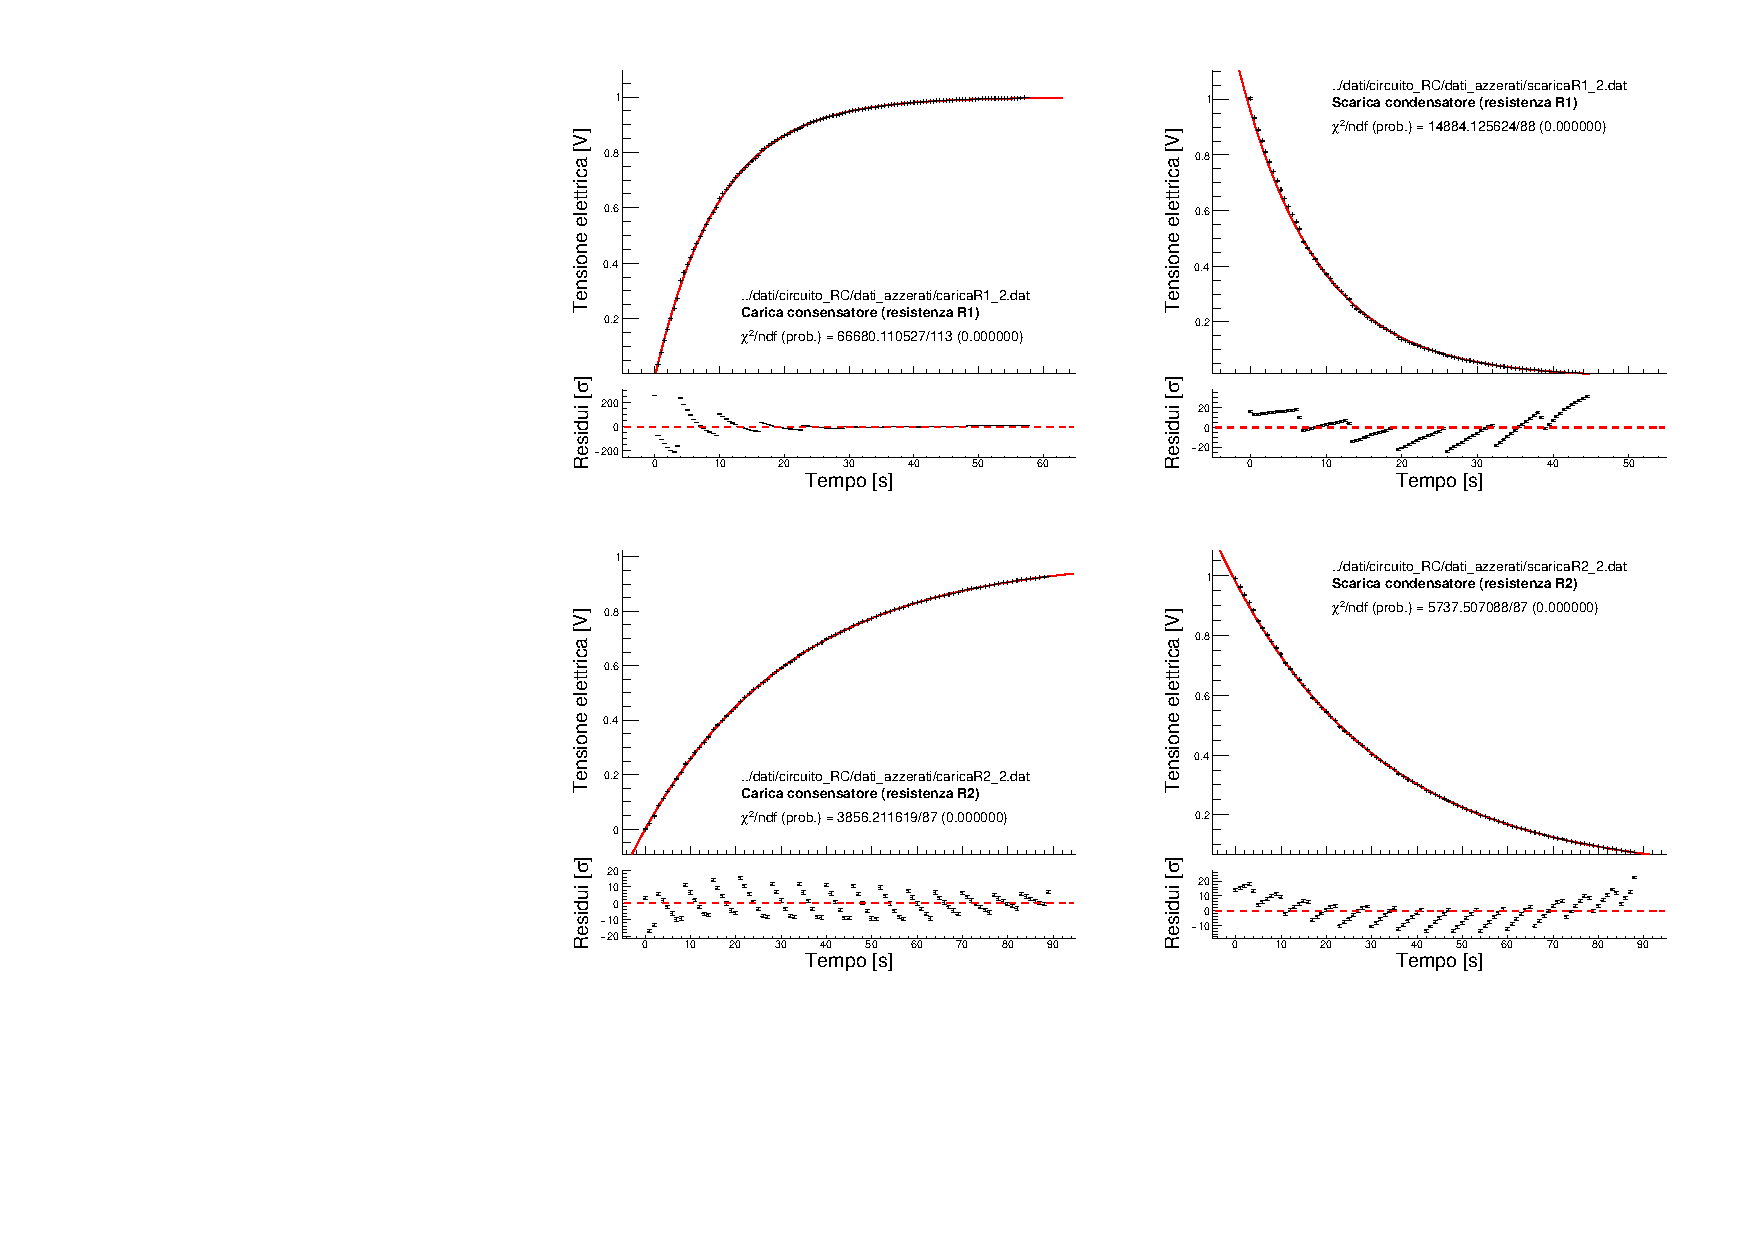
\includegraphics[width=\linewidth]{plot_RC.pdf}
        \caption{Rappresentazione del processo di carica e scarica del condensatore in presenta di resistenza $R_1$ (sopra) e $R_2$ (sotto). }
        \label{figure:plot_RC}
    \end{figure*}

    Dai file raccolti dal software DMMDaq riportati nell'appendice \ref{section:appendix_EXT_DATA} rappresentiamo in \reffig{figure:plot_RC} le coppie ($t$, $V_C(t)$) per i processi di carica e scarica relativi alle due resistenze. \\
    L'errore relativo a $t$ si assume essere $\mstdErr{t}=0.005\cdot T$ dove $T=\Delta t$ è l'intervallo che intercorre tra due misurazioni. Per l'errore relativo a $V_C$ consideriamo la maggiore tra le seguenti quantità: 
    \[
        \mstdErr{V_C} = \frac{1}{\sqrt{12}}\left|V_{(i)}-V_{(i-1)}\right|\frac{0.3~\text{s}}{T}  
    \]oppure l'incertezza deducibile dal data-sheet dello strumento
    \[
        \mstdErr{V_C}=\frac{0.015\% \cdot val + 0.003\% * range}{\sqrt{3}}~~~(\text{range}=2~\text{V}).
    \]

    Sui punti rappresentati in \reffig{figure:plot_RC} eseguiamo poi fit utilizzando la \refeqn{equation:carica} per i processi di carica (\reffig{figure:plot_RC} a sinistra, sopra con la resistenza $R_1$ sotto $R_2$), e la \refeqn{equation:scarica} per i processi di scarica (\reffig{figure:plot_RC} a destra, sopra con la resistenza $R_1$ sotto $R_2$).

    Dai modelli di Fit ricaviamo i valori di $V_\infty\pm\mstdErr{V_\infty}$, $\tau\pm\mstdErr{\tau}$ e $t_0\pm\mstdErr{t_0}$ per il processo di carica, $V_0\pm\mstdErr{V_0}$ e $\tau\pm\mstdErr{\tau}$ per il processo di scarica.

    Da questi valori, in particolar modo dal valore di $\tau$, possiamo ricavare la capacità C del condensatore. Infatti se $\tau=RC$, otteniamo che \[C=\frac{\tau}{R},\] da cui otteniamo che \[\mstdErr{C}=C\sqrt{\left(\frac{\mstdErr{\tau}}{\tau}\right)^2+\left(\frac{\mstdErr{R}}{R}\right)^2}.\]

    \section{Risultati}
    \label{section:results}

    Dal fit eseguito su \refeqn{equation:VI} ricaviamo i valori delle resistenze $R_1$ e $R_2$, e dell'intercetta. Ritroviamo quindi i valori $R_1^s=(9.911\pm0.033)$~k$\Omega$ e $R_2^s=(32.65\pm0.13)$~k$\Omega$. Osserviamo che le resistenze sono compatibili con i valori misurati in laboratorio, infatti 
    \[\left|R_1^s-R_1^m\right|=0.026<0.981=3\sqrt{\mstdErr{R_1^s}^2+\mstdErr{R_1^m}^2}\]
    e analogamente
    \[\left|R_2^s-R_2^m\right|=0.118<0.391=3\sqrt{\mstdErr{R_2^s}^2+\mstdErr{R_2^m}^2}\]
    
    Inoltre come anche indicato nel listato in \autoref{section:appendix_EXT_DATA}, osserviamo che in entrambi i casi le intercette sono compatibili con il valore di zero.

    Prendiamo ora invece in considerazione i risultati ottenuti dai Fit di \refeqn{equation:carica} e \refeqn{equation:scarica} e rappresentati in \reffig{figure:plot_RC}. 

    Per i processi di carica otteniamo i seguenti valori:
    \begin{itemize}
        \item con la resistenza $R_1$:
        \begin{itemize}
            \item il valore di $V_\infty^{R_1}=(0.999259\pm0.000020)$~V, 
            \item il valore di $\tau^{R_1}_{\text{carica}}=(10.0453\pm0.0012)$~s, 
            \item il valore di $t_0^{R_1}=(0.1137\pm0.0009)$~s;
        \end{itemize}
        \item con la resistenza $R_2$:
        \begin{itemize}
            \item il valore di $V_\infty^{R_2}=(0.99698\pm0.00008)$~V,
            \item il valore di $\tau^{R_2}_{\text{carica}}=(10.0453\pm0.0012)$~s,
            \item il valore di $t_0^{R_2}=(0.1137\pm0.0009)$~s;
        \end{itemize}
    \end{itemize}
    
    Per i processi di scarica otteniamo invece i seguenti valori:
    \begin{itemize}
        \item con la resistenza $R_1$:
        \begin{itemize}
            \item il valore di $V_0^{R_1}=(0.9542\pm0.0004)$~V, 
            \item il valore di $\tau^{R_1}_{\text{scarica}}=(10.5437\pm0.0018)$~s, 
        \end{itemize}
        \item con la resistenza $R_2$:
        \begin{itemize}
            \item il valore di $V_0^{R_2}=(0.97982\pm0.00017)$~V,
            \item il valore di $\tau^{R_2}_{\text{scarica}}=(34.021\pm0.004)$~s,
        \end{itemize}
    \end{itemize}

    Dai valori di $\tau$ otteniamo i valori di $C\pm\mstdErr{C}$:
    \begin{itemize}
        \item da $\tau^{R_1}_{\text{carica}}$ e $R_1^s$ otteniamo $C_0=(1.016\pm0.003)$~mF,
        \item da $\tau^{R_1}_{\text{scarica}}$ e $R_1^s$ otteniamo $C_1=(1.064\pm0.004)$~mF,
        \item da $\tau^{R_2}_{\text{carica}}$ e $R_2^s$ otteniamo $C_2=(1.021\pm0.004)$~mF,
        \item da $\tau^{R_2}_{\text{scarica}}$ e $R_2^s$ otteniamo $C_3=(1.041\pm0.004)$~mF,
    \end{itemize}

    Con l'utilizzo di \cernroot e di semplici algoritmi verifichiamo la compatibilità dei valori ottenuti, e, come indicato in fondo al listato di output, osserviamo che vi è compatibilità solo tra $C_0$ e $C_2$.

    \section{Conclusione}
    \label{section:conclusion}

    Osserviamo che i valori del rapporto \ChiNdf~ per la prima parte della esperienza è molto basso, e la probabilità del \ChiSqr~ è estremamente alta, tanto da farci ipotizzare che gli errori sulle tensioni siano stati sovrastimati. Lo strumento utilizzato infatti è uno stato progettato per poter operare in una più ampia gamma di condizioni di misura, e questo al costo di perdere accuratezza.

    Nonostante ciò osserviamo un andamento lineare in accordo con la teoria.
    Inoltre troviamo che entro \treSigma~ i valori sono compatibili con la misura diretta effettuata in laboratorio.

    La seconda parte della esperienza presenta invece molte problematiche che di seguito ci impegniamo a commentare.

    Infatti solo osservando i valori di \ChiNdf~ e la probabilità del \ChiSqr, possiamo notare come il risultato non sia compatibile con la teoria, e mostri uno scostamento significativo (ben superiore $5\sigma$).

    Già durante la presa dati abbiamo potuto osservare che i punti rappresentati nel software DMMDaq presentavano un andamento discontinuo, che è stato confermato da una successiva analisi dati dettagliata. Infatti questo problema viene reso più evidente nell'analisi dei residui in \reffig{figure:plot_RC} dove osserviamo che i punti, oltre a essere distanti dalla miglior retta oltre $50\sigma$, presenta un andamento particolare, dove a periodi di circa 8~s i dati presentano uno salto.

    Osservando meglio il grafico inoltre sembra come se a blocchi di 8~s i punti debbano essere circa traslati rigidamente avanti di un certo $\Delta t$ ignoto.
    
    Riteniamo che questo fatto possa essere dovuto ad un problema di acquisizione dati: il multimetro da banco  utilizzato per effettuare le misurazioni, e il computer utilizzato per la raccolta dati potrebbero non essere perfettamente sincronizzati. Questo potrebbe causare la perdita cadenzata di un dato ogni “n” acquisizioni di dati(circa ogni 8 secondi). Graficamente il risultato è lo shift su un certo lasso di tempo della distribuzione dei dati.

    L'ipotesi che questo $\Delta t$ equivalga a esattamente una variazione tra il tempo di presa dati di due punti è stata inizialmente presa in considerazione, e abbiamo eseguito una prova dove a blocchi di 8 secondi, stando attenti a spostare i punti in prossimità del salto. Questa ipotesi nasce dal fatto che se il computer avesse saltato un periodo avrebbe associato il valore della $V$ successiva al periodo precedente, causando questo sfasamento. Questa ipotesi è stata poi scartata in seguito ad una prova dove il risultato non variava significativamente. Segue che l'idea che ci possa essere un offset temporale $\Delta t$ sia probabile, ma che tale $\Delta t$ non sia costante e neanche ricavabile dai dati.

    Da questi problemi legati al fit dei dati per la seconda parte segue inoltre che la non compatibilità dei valori di capacità $C$ sia giustificata.

    \appendix

    \setcounter{table}{0}
    \renewcommand{\thetable}{A\arabic{table}}

    \section{Dati aggiuntivi}
    \label{section:appendix_EXT_DATA}

    Per la seconda parte dell'esperienza sono stati utilizzati i file \verb|caricaR1_2.dat|, \verb|caricaR2_2.dat|, \verb|scaricaR1_2.dat| e \verb|scaricaR2_2.dat| posti nella cartella \verb|./dati/circuito_RC/dati_azzerati/|.

    Aggiungiamo di seguito il listato di output di \cernroot, utilizzato nell versione \verb|6.22/06|.
    {\fontsize{6}{6}
\begin{verbatim}
**********
   METODO VOLT-AMPEROMETRICO PER RICAVARE R1 E R2
**********

FCN=0.148025 FROM MIGRAD    STATUS=CONVERGED      45 CALLS          46 TOTAL
                    EDM=2.74849e-08    STRATEGY= 1      ERROR MATRIX ACCURATE 
 EXT PARAMETER                                   STEP         FIRST   
 NO.   NAME      VALUE            ERROR          SIZE      DERIVATIVE 
  1  p0          -3.48275e-04   4.12547e-03   1.66617e-06  -9.84148e-03
  2  p1           9.91087e-03   3.26730e-05   1.31958e-08  -7.90133e+00

** CHI2 / NDF ( PROB. ) 0.148025 / 5 ( 0.999575 )

** COMPATIBILITA' DI ZERO PER R0 => COMPATIBILE

FCN=0.0638172 FROM MIGRAD    STATUS=CONVERGED      50 CALLS          51 TOTAL
                    EDM=3.03492e-14    STRATEGY= 1      ERROR MATRIX ACCURATE 
 EXT PARAMETER                                   STEP         FIRST   
 NO.   NAME      VALUE            ERROR          SIZE      DERIVATIVE 
  1  p0          -6.86019e-04   7.62488e-03   2.47655e-06  -3.44546e-05
  2  p1           3.26516e-02   1.27408e-04   4.13820e-08  -1.71995e-04

** CHI2 / NDF ( PROB. ) 0.0638172 / 5 ( 0.999947 )

** COMPATIBILITA' DI ZERO PER R1 => COMPATIBILE


**********
   CONTROLLO COMPATIBILITA' R1 E R2
**********

** R1 => COMPATIBILE
R1 (misurata) 9.9371 +/- 0.00149385 kOhm
R1 (ricavata) 9.91087 +/- 0.032673 kOhm

** R2 => COMPATIBILE
R2 (misurata) 32.77 +/- 0.00724806 kOhm
R2 (ricavata) 32.6516 +/- 0.127408 kOhm


**********
   STUDIO CIRCUITO RC
**********

** READING FROM FILE ../dati/circuito_RC/dati_azzerati/caricaR1_2.dat

FCN=66680.1 FROM MINOS     STATUS=SUCCESSFUL     16 CALLS         169 TOTAL
                    EDM=2.88727e-08    STRATEGY= 1      ERROR MATRIX ACCURATE 
 EXT PARAMETER                                   STEP         FIRST   
 NO.   NAME      VALUE            ERROR          SIZE      DERIVATIVE 
  1  p0           9.99259e-01   2.00376e-05   0.00000e+00   1.72605e+01
  2  p1           1.00453e+01   1.24891e-03   0.00000e+00  -6.13545e-01
  3  p2           1.13656e-01   8.78720e-04   8.78720e-04  -1.95730e-01

** CHI2 / NDF ( PROB. ) 66680.1 / 113 ( 0 )

V_0/V_I 0.999259 +/- 2.00376e-05 V
tau     10.0453 +/- 0.00124891 s

** COMPATIBILITA' DI ZERO =>NON-COMPATIBILE
t_0     0.113656 +/- 0.00087872 s

** READING FROM FILE ../dati/circuito_RC/dati_azzerati/scaricaR1_2.dat

FCN=14884.1 FROM MINOS     STATUS=SUCCESSFUL     12 CALLS          89 TOTAL
                    EDM=2.22382e-08    STRATEGY= 1      ERROR MATRIX ACCURATE 
 EXT PARAMETER                                   STEP         FIRST   
 NO.   NAME      VALUE            ERROR          SIZE      DERIVATIVE 
  1  p0           9.54209e-01   4.12175e-04   6.75828e-08  -4.98710e-03
  2  p1           1.05437e+01   1.84963e-03   1.84963e-03  -1.25465e-03

** CHI2 / NDF ( PROB. ) 14884.1 / 88 ( 0 )

V_0/V_I 0.954209 +/- 0.000412175 V
tau     10.5437 +/- 0.00184963 s

** READING FROM FILE ../dati/circuito_RC/dati_azzerati/caricaR2_2.dat

FCN=3856.21 FROM MINOS     STATUS=SUCCESSFUL     40 CALLS         254 TOTAL
                    EDM=6.04053e-10    STRATEGY= 1      ERROR MATRIX ACCURATE 
 EXT PARAMETER                                   STEP         FIRST   
 NO.   NAME      VALUE            ERROR          SIZE      DERIVATIVE 
  1  p0           9.96983e-01   7.52169e-05  -2.48891e-07  -2.63551e-01
  2  p1           3.33239e+01   9.48424e-03  -4.19678e-05   2.62352e-03
  3  p2           3.44903e-02   4.95656e-03   4.95656e-03  -1.48931e-02

** CHI2 / NDF ( PROB. ) 3856.21 / 87 ( 0 )

V_0/V_I 0.996983 +/- 7.52169e-05 V
tau     33.3239 +/- 0.00948424 s

** COMPATIBILITA' DI ZERO =>NON-COMPATIBILE
t_0     0.0344903 +/- 0.00495656 s

** READING FROM FILE ../dati/circuito_RC/dati_azzerati/scaricaR2_2.dat

FCN=5181.59 FROM MINOS     STATUS=SUCCESSFUL     12 CALLS          97 TOTAL
                    EDM=8.39373e-10    STRATEGY= 1      ERROR MATRIX ACCURATE 
 EXT PARAMETER                                   STEP         FIRST   
 NO.   NAME      VALUE            ERROR          SIZE      DERIVATIVE 
  1  p0           9.80445e-01   1.74132e-04   3.07311e-08  -4.63678e-03
  2  p1           3.39966e+01   4.02596e-03   4.02596e-03  -3.38165e-04

** CHI2 / NDF ( PROB. ) 5181.59 / 87 ( 0 )

V_0/V_I 0.980445 +/- 0.000174132 V
tau     33.9966 +/- 0.00402596 s


**********
   STIMA DELLA CAPACITA' C 
**********

C (da carica R1)  1.01357 +/- 0.00334379 mF
C (da scarica R1) 1.06385 +/- 0.00351215 mF
C (da carica R2)  1.02059 +/- 0.00399299 mF
C (da scarica R2) 1.04119 +/- 0.00406466 mF

** COMPATIBILITA' TRA C[0] E C[1] => NON-COMPATIBILE
** COMPATIBILITA' TRA C[0] E C[2] => COMPATIBILE
** COMPATIBILITA' TRA C[0] E C[3] => NON-COMPATIBILE
** COMPATIBILITA' TRA C[1] E C[0] => NON-COMPATIBILE
** COMPATIBILITA' TRA C[1] E C[2] => NON-COMPATIBILE
** COMPATIBILITA' TRA C[1] E C[3] => NON-COMPATIBILE
** COMPATIBILITA' TRA C[2] E C[0] => COMPATIBILE
** COMPATIBILITA' TRA C[2] E C[1] => NON-COMPATIBILE
** COMPATIBILITA' TRA C[2] E C[3] => NON-COMPATIBILE
** COMPATIBILITA' TRA C[3] E C[0] => NON-COMPATIBILE
** COMPATIBILITA' TRA C[3] E C[1] => NON-COMPATIBILE
** COMPATIBILITA' TRA C[3] E C[2] => NON-COMPATIBILE

\end{verbatim}
}
    

\end{document}
    
